\section{Design architetturale}

Il gruppo ha scelto di lasciare la libreria non vincolata da dipendenze esterne oltre alla scelta del linguaggio Scala, dettata dai requisiti.
%
Non sono infatti state utilizzate librerie esterne se non quelle per il testing automatizzato.

% ---------------------------------------------------

\subsection{Pattern architetturali}

Data la natura del progetto è risultato necessario fornire delle astrazioni ben consolidate.
%
In particolare, per applicazioni che si basano sull'interazione utente, il pattern \textbf{MVC} è uno dei più noti e flessibili.

La separazione delle responsabilità fra i vari componenti è uno dei motivi principali per cui è stato scelto questo pattern: è infatti possibile per un utente della libreria descrivere totalmente un gioco senza fare alcun riferimento alla sua rappresentazione, e solo successivamente collegare ad esso interazione e visualizzazione.
%
Questo è di particolare importanza in una libreria come SBAGS, in quanto diversi tipi di interfaccia potrebbero essere necessari per diversi tipi di giochi, e correlare presentazione a modello lo renderebbe più complesso e dispendioso.

Un'ulteriore motivazione risiede nell'abilitare la possibilità di fornire più modalità di visualizzazione del gioco e di interpretazione dell'input utente che possano essere direttamente utilizzabili dagli utenti della libreria.

% ---------------------------------------------------

\subsection{Architettura complessiva}

L'interpretazione del pattern MVC adottata in questo progetto è basata su gerarchie di controller e di view: ogni fase dell'applicazione -- es. menu, partita in corso -- ha una sua coppia di view e controller che gestiscono la specifica situazione.

\subsubsection{Utilizzo del pattern MVC}

Come mostrato in Figura \ref{fig:main_class_diagram} è possibile, tramite l'interfaccia \texttt{View} principale, generare le \texttt{SubView} a cui associare i vari \texttt{SubController}.
%
\begin{figure}
  \centering
  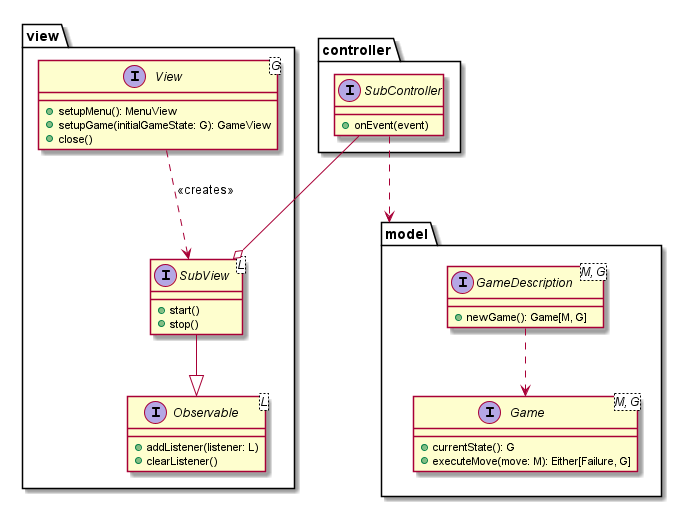
\includegraphics[width=\linewidth]{images/uml/main_class_diagram.png}
  \caption{Diagramma rappresentante le principali interfacce di model, view e controller}
  \label{fig:main_class_diagram}
\end{figure}
%
Si noti che il concetto di \texttt{SubController} presente nel diagramma non è stato effettivamente materializzato nel codice, ma è stato utilizzato per semplificare la lettura dello schema e della relativa prosa.

Ogni \texttt{SubView} specifica quale deve essere l'interfaccia del proprio tipo di listener, che viene poi implementata dal \texttt{SubController} corrispondente.
%
Quest'ultimo incapsula la logica di business della \texttt{SubView} a cui è associato e di conseguenza governa il passaggio da una \texttt{SubView} all'altra.

I listener, dopo essere stati aggiunti, vengono notificati seguendo il pattern \textbf{Observer}, in base agli eventi che accadono alla relativa \texttt{SubView}.

\subsubsection{Navigazione delle SubView}

L'architettura supporta la navigazione tra le sotto viste grazie all'interfaccia principale della View.
%
Il processo per eseguire un passaggio a una nuova \texttt{SubView} è descritto in Figura \ref{fig:view_navigation}.
%
In questo caso è stato mostrato quello relativo alla \texttt{MenuView}, ma i concetti sono generalizzabili a qualsiasi altra vista.
%
\begin{figure}
  \centering
  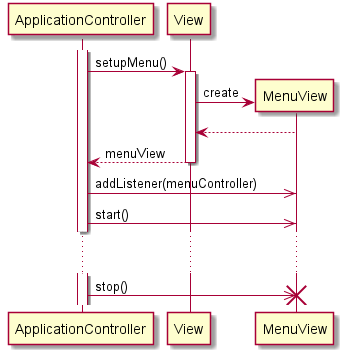
\includegraphics[width=0.6\linewidth]{images/uml/view_navigation.png}
  \caption{Interazioni necessarie per la navigazione tra SubView}
  \label{fig:view_navigation}
\end{figure}

L'interazione ha inizio generalmente da un controller, che richiede alla \texttt{View} una nuova istanza della \texttt{SubView} che vuole visualizzare.
%
In questo momento la \texttt{SubView} non è ancora visibile, per permettere al controller di registrare i listener necessari.
%
Per fare in modo che sia visibile, il controller deve richiamare il metodo \texttt{start}.

La modalità scelta per la navigazione prevede che ci sia uno \textbf{stack} di \texttt{SubView} attive in un dato momento.
%
Questo significa che ogni volta che viene aperta una nuova visualizzazione, quella precedente non viene chiusa, ma resta inattiva.
%
Quando quest'ultima viene chiusa (tramite il metodo \texttt{stop}), quella che era stata disattivata riprende il controllo e diventa la view attiva.
